\section{The almond: skeleton sources and a tip tail}
\label{sec:almond}

The NASA almond \cite{woo1993} is a standard target for radar cross-section codes. It is a smooth body of length $L = 0.2524$\,m ($9.936$\,in) with a rounded rear and a sharp tip. Every cross-section is an ellipse with axis ratio $3:1$. We place the almond with its long axis along $x$, the tip at positive $x$ and its mid-plane in $z = 0$. It is symmetric under the mirrors $y\to-y$ and $z\to-z$.

\subsection{Sources}

By \autoref{sec:skeleton} the sources lie on the mid-plane and cluster towards the focal curve, which runs at the fraction $\eta_F = 0.943$ of the half-width (\autoref{fig:almondlayout}). They are point dipoles arranged in rows. A row follows the outline of the mid-plane section at a fixed fraction $\eta$ of the half-width. We use $n_{\mathrm{mid}}$ rows in the middle of the section and $J+1$ rows at
\begin{equation}
  \eta_j = \eta_F - 2\,(1-\eta_F)\,2^{-j}, \qquad j = 0,\dots,J,
\end{equation}
which approach the focal curve geometrically from the inside. Along a row the spacing of the sources is a fixed multiple $s$ of the local distance to the surface. The collocation points on the surface follow the same rule, so that sources and collocation points refine together towards the rim. We write $n_{\mathrm{mid}}{:}J$ for a layout.

A source on a mirror plane of a field of definite parity keeps only three of its six dipole components. For fields that are even under $z\to-z$ these are the electric components $a_x$, $a_y$ and the magnetic component $m_z$. For odd fields they are $a_z$, $m_x$ and $m_y$. Each source therefore carries three unknowns. As for the cube, an incident wave is split into its parts of definite parity under the two mirrors. Each of the four classes is solved with the sources and collocation points of one quarter of the body.

\begin{figure}[htbp]
  \centering
  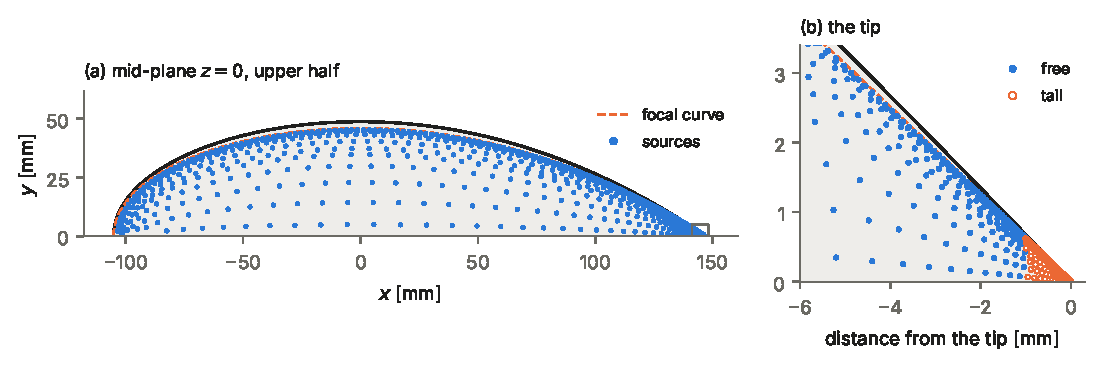
\includegraphics[width=0.9\textwidth]{fig_almond_layout.pdf}
  \caption{Source layout of the almond in the mid-plane $z = 0$ (one half shown). The rows of point dipoles cluster towards the focal curve (dashed), which runs within $6\%$ of the rim, and continue into the tip as a tail.}
  \label{fig:almondlayout}
\end{figure}

\subsection{The tip}

The focal curve reaches the surface at the tip, which is the vertex of an elliptic cone with half-angles $34.09^\circ$ and $12.71^\circ$. The field of a conducting cone behaves like $r^{\nu-1}$ at distance $r$ from the vertex. For this cone the smallest exponent is $\nu = 0.29959$ (\ref{app:cone}), so the electric field grows like $r^{-0.70}$. This singular term belongs to the class that is even under both mirrors, which is the class that drives current along the axis into the tip. In the other three classes all exponents exceed $0.87$.

The free source rows stop $1$\,mm from the tip. For the class that is even under both mirrors this cut-off leaves a boundary residual of $19\%$, half of it within $1$\,mm of the tip. The cross-section at oblique angles is then wrong by up to $1.2$\,dB. Adding sources does not help. The remedy is the tail of \autoref{sec:cube}. Each row is continued to within $10^{-4}$\,mm of the tip with the same spacing rule. The continued dipoles of a row are tied together with the weights $(r/r_{\mathrm{cut}})^{e}$, where $e = \nu+2$ for electric and $e = \tau+2$ for magnetic dipoles. With the tail and the spacing $s = 0.5$ the residual of this class falls to $0.23\%$, and with $s = 0.4$ to $0.034\%$. The other classes are converged at $s = 0.7$.

Before we computed the exponents of the cone we had fitted a set of four exponents between $2.2$ and $3.0$. The single computed value $e = 2.29959$ gives the same residual, and the fitted set is no longer needed.

\subsection{Nose-on incidence at 1.19 GHz}

We first consider the wave that travels along $-x$ towards the tip, polarised along $y$, at $1.19$\,GHz, where the almond is one wavelength long. \autoref{tab:almond} and \autoref{fig:costalmond} show the difference from the finest layout, $8{:}5$ with $4791$ unknowns. This reference is itself converged: a closer spacing along the rows ($s = 0.5$), a finer collocation grid, and twice as many rows towards the focal curve each change its field by less than $10^{-5}$. The layouts $5{:}2$ and $6{:}3$ reach $2.8\times10^{-4}$ and $5.6\times10^{-5}$ in $2.1$ and $3.2$\,s. Bempp reaches $3.0\times10^{-3}$ with $9558$ unknowns in $19$\,s, and its error is inversely proportional to the number of unknowns. At an error of one per cent the two methods take about the same time, one second. The MFS uses the two mirror symmetries of this wave, which Bempp does not.

\begin{table}[htbp]
  \centering
  \caption{NASA almond, $1.19$\,GHz, nose-on incidence: unknowns, wall time and difference from the finest MFS layout.}
  \label{tab:almond}
  \begin{tabular}{lrrl}
    \toprule
    Method & Unknowns & Time [s] & Error \\
    \midrule
\tablebody{almond}
    \bottomrule
  \end{tabular}
\end{table}

\begin{figure}[htbp]
  \centering
  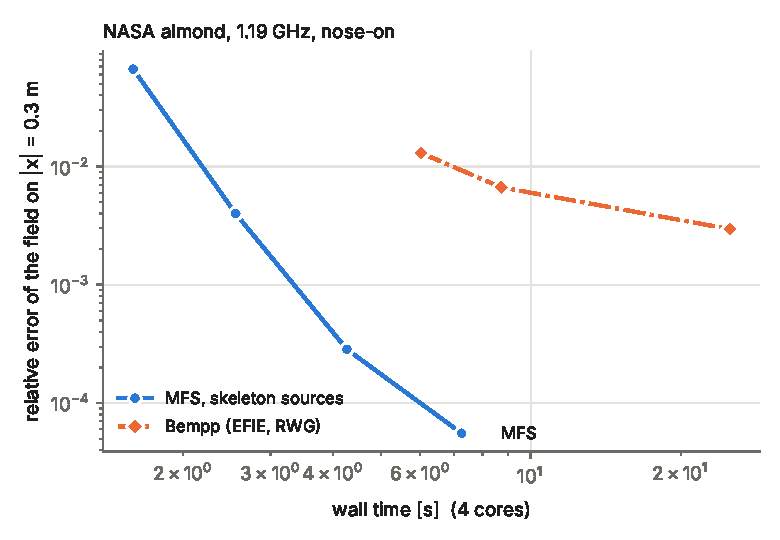
\includegraphics[width=0.62\textwidth]{fig_cost_almond.pdf}
  \caption{NASA almond, $1.19$\,GHz, nose-on incidence: difference from the finest MFS layout against wall time on four cores.}
  \label{fig:costalmond}
\end{figure}

\subsection{Monostatic radar cross-section}

The quantity of practical interest is the monostatic cross-section as a function of the azimuth in the plane of the almond, for the polarisations HH (electric field in the plane) and VV (electric field along $z$). HH needs the two classes that are even in $z$ and VV the two that are odd. The factorisation of a class serves all look angles. One frequency, with $361$ look angles and both polarisations, takes $66$\,s with the layout $6{:}3$.

We compare with the Austin RCS Benchmark Suite \cite{kelley2020}, which provides measurements of this almond and a reference simulation on a fine mesh at $3.5$, $5.125$, $7$ and $10.25$\,GHz. At the highest frequency the almond is $8.6$ wavelengths long. \autoref{fig:almondbench} shows the three sets of curves, and \autoref{tab:almondbench} lists the mean absolute difference in decibels over the $361$ look angles. The MFS differs from the reference simulation by $0.04$ to $0.14$\,dB for HH and by $0.01$ to $0.02$\,dB for VV. Both simulations differ from the measurements by $0.6$ to $1.8$\,dB, and the two distances agree to within $0.07$\,dB in every case.
%% TODO: quote the measurement uncertainty from Kelley et al. once the paper is at hand.

\begin{table}[htbp]
  \centering
  \caption{NASA almond, monostatic cross-section: mean absolute difference in dB between the MFS (layout $6{:}3$) and the reference simulation of the Austin benchmark \cite{kelley2020}, over $361$ look angles.}
  \label{tab:almondbench}
  \begin{tabular}{lrrrr}
    \toprule
    Frequency [GHz] & 3.5 & 5.125 & 7 & 10.25 \\
    \midrule
    HH & 0.043 & 0.055 & 0.072 & 0.140 \\
    VV & 0.011 & 0.013 & 0.016 & 0.024 \\
    \bottomrule
  \end{tabular}
\end{table}

\begin{figure}[htbp]
  \centering
  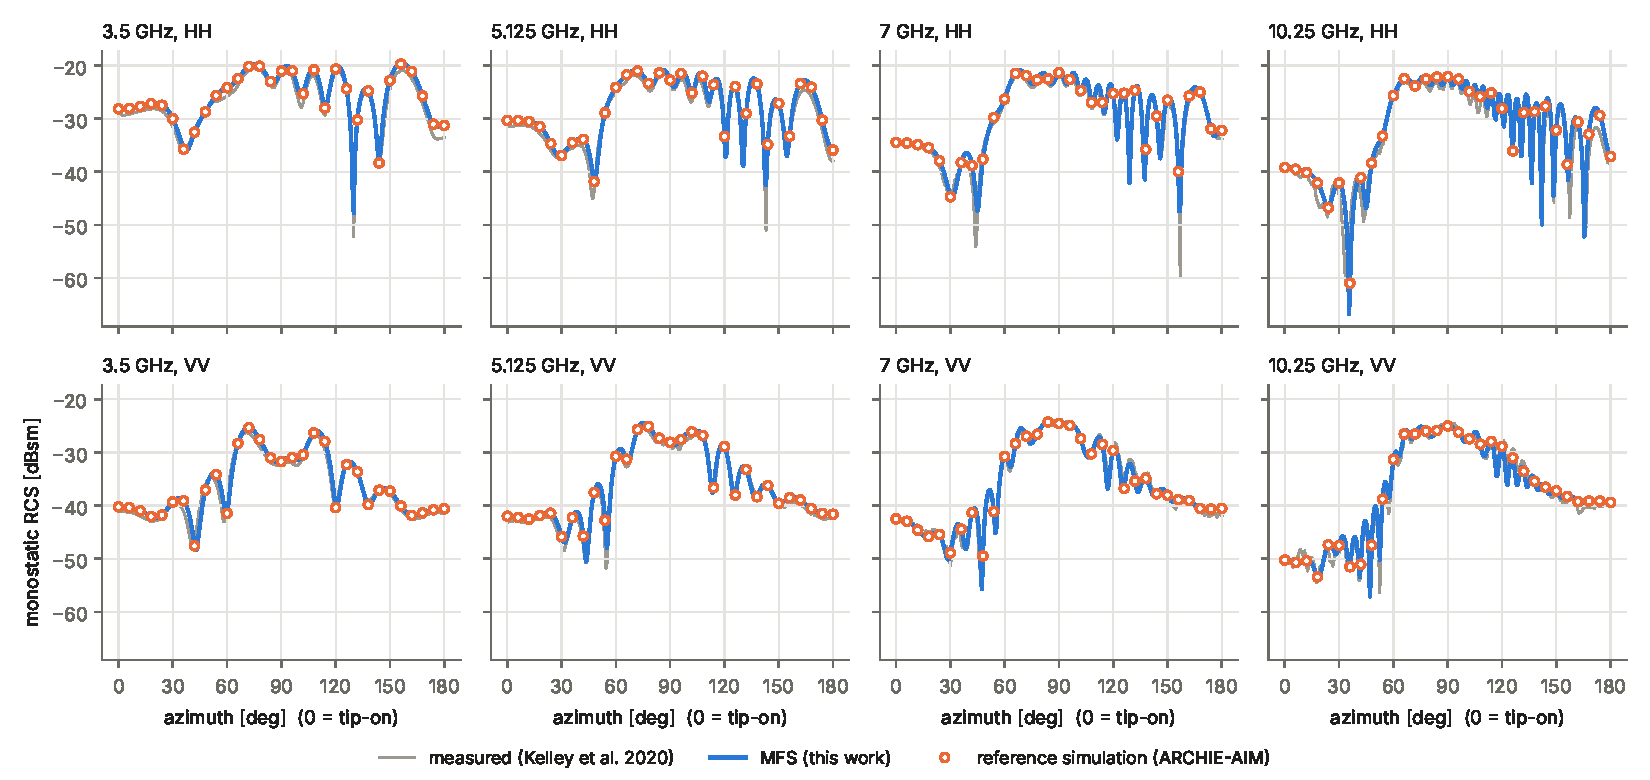
\includegraphics[width=\textwidth]{fig_almond_benchmark.pdf}
  \caption{NASA almond: monostatic radar cross-section against azimuth ($0^\circ$ is nose-on) at four frequencies, HH and VV. MFS, reference simulation and measurements of the Austin benchmark \cite{kelley2020}.}
  \label{fig:almondbench}
\end{figure}

The largest pointwise differences from the reference simulation occur in deep nulls of the HH cross-section. The largest is $4.3$\,dB at $10.25$\,GHz and $35.5^\circ$, in a null at $-66.7$\,dBsm. The MFS is converged there: the layouts $6{:}3$ and $8{:}5$ differ by $0.0006$\,dB on average and by $0.024$\,dB in this null.
The difference is one of position, not of depth. On a grid of $0.02^\circ$ the MFS places this null at $35.66^\circ$ with a depth of $-69.7$\,dBsm, and the cross-section rises by $8$ to $12$\,dB within half a degree on either side. The reference data are sampled every $0.5^\circ$. Shifting the MFS curve by $0.1^\circ$ halves its distance from the reference samples around the null. A shift of this size corresponds to a change of $0.05\%$ in the size of the almond or in the frequency. We conclude that the two simulations agree on this null to within a tenth of a degree, and that the $4.3$\,dB is the price of sampling a sharp null.

At $1.19$, $7$ and $9.92$\,GHz we also compared with Bempp on meshes with $9558$ and $13632$ unknowns. The root-mean-square differences are $0.02$, $0.04$ and $0.12$\,dB for HH and $0.03$, $0.03$ and $0.09$\,dB for VV. At $1.19$\,GHz the MFS cross-section changes by $0.001$\,dB when the row spacing is reduced from $0.5$ to $0.4$.
